\chapter{中子扩散理论与计算}
\section*{习题}

\begin{exercise}
    试总结中子扩散理论的适用范围。
    \begin{solution}
        \begin{enumerate}[(1)]
            \item 有限介质内距表面几个自由程之外的内部区域,即满足无限介质假设;
            \item 在距强吸收体几个自由程之外的区域,即满足弱吸收假设;
            \item 在距中子源几个自由程之外或两种扩散性质差异显著的介质交界面几个自由程之外的区域,即满足中子通量密度缓慢变化。
        \end{enumerate}
    \end{solution}
\end{exercise}

\begin{exercise}
    有两束方向相反的平行热中子束射到${}^{235}\symrm{U}$薄片上,设其上某点自左面人射的中子束强度为$10^{12}\,\symrm{cm^2\cdot s^{-1}}$,自右面人射的中子束强度$2 \times 10^{12}\,\symrm{cm^2\cdot s^{-1}}$。计算:
    \begin{enumerate}[(1)]
        \item 该点的中子注量率;
        \item 该点的中子流密度;
        \item 设$\vSigma_{\symrm{a}} = 19.2 \times 10^2\,\symrm{m^{-1}}$,求该点的吸收率。
    \end{enumerate}
    \begin{solution}
        \begin{figure}[H]
            \centering
            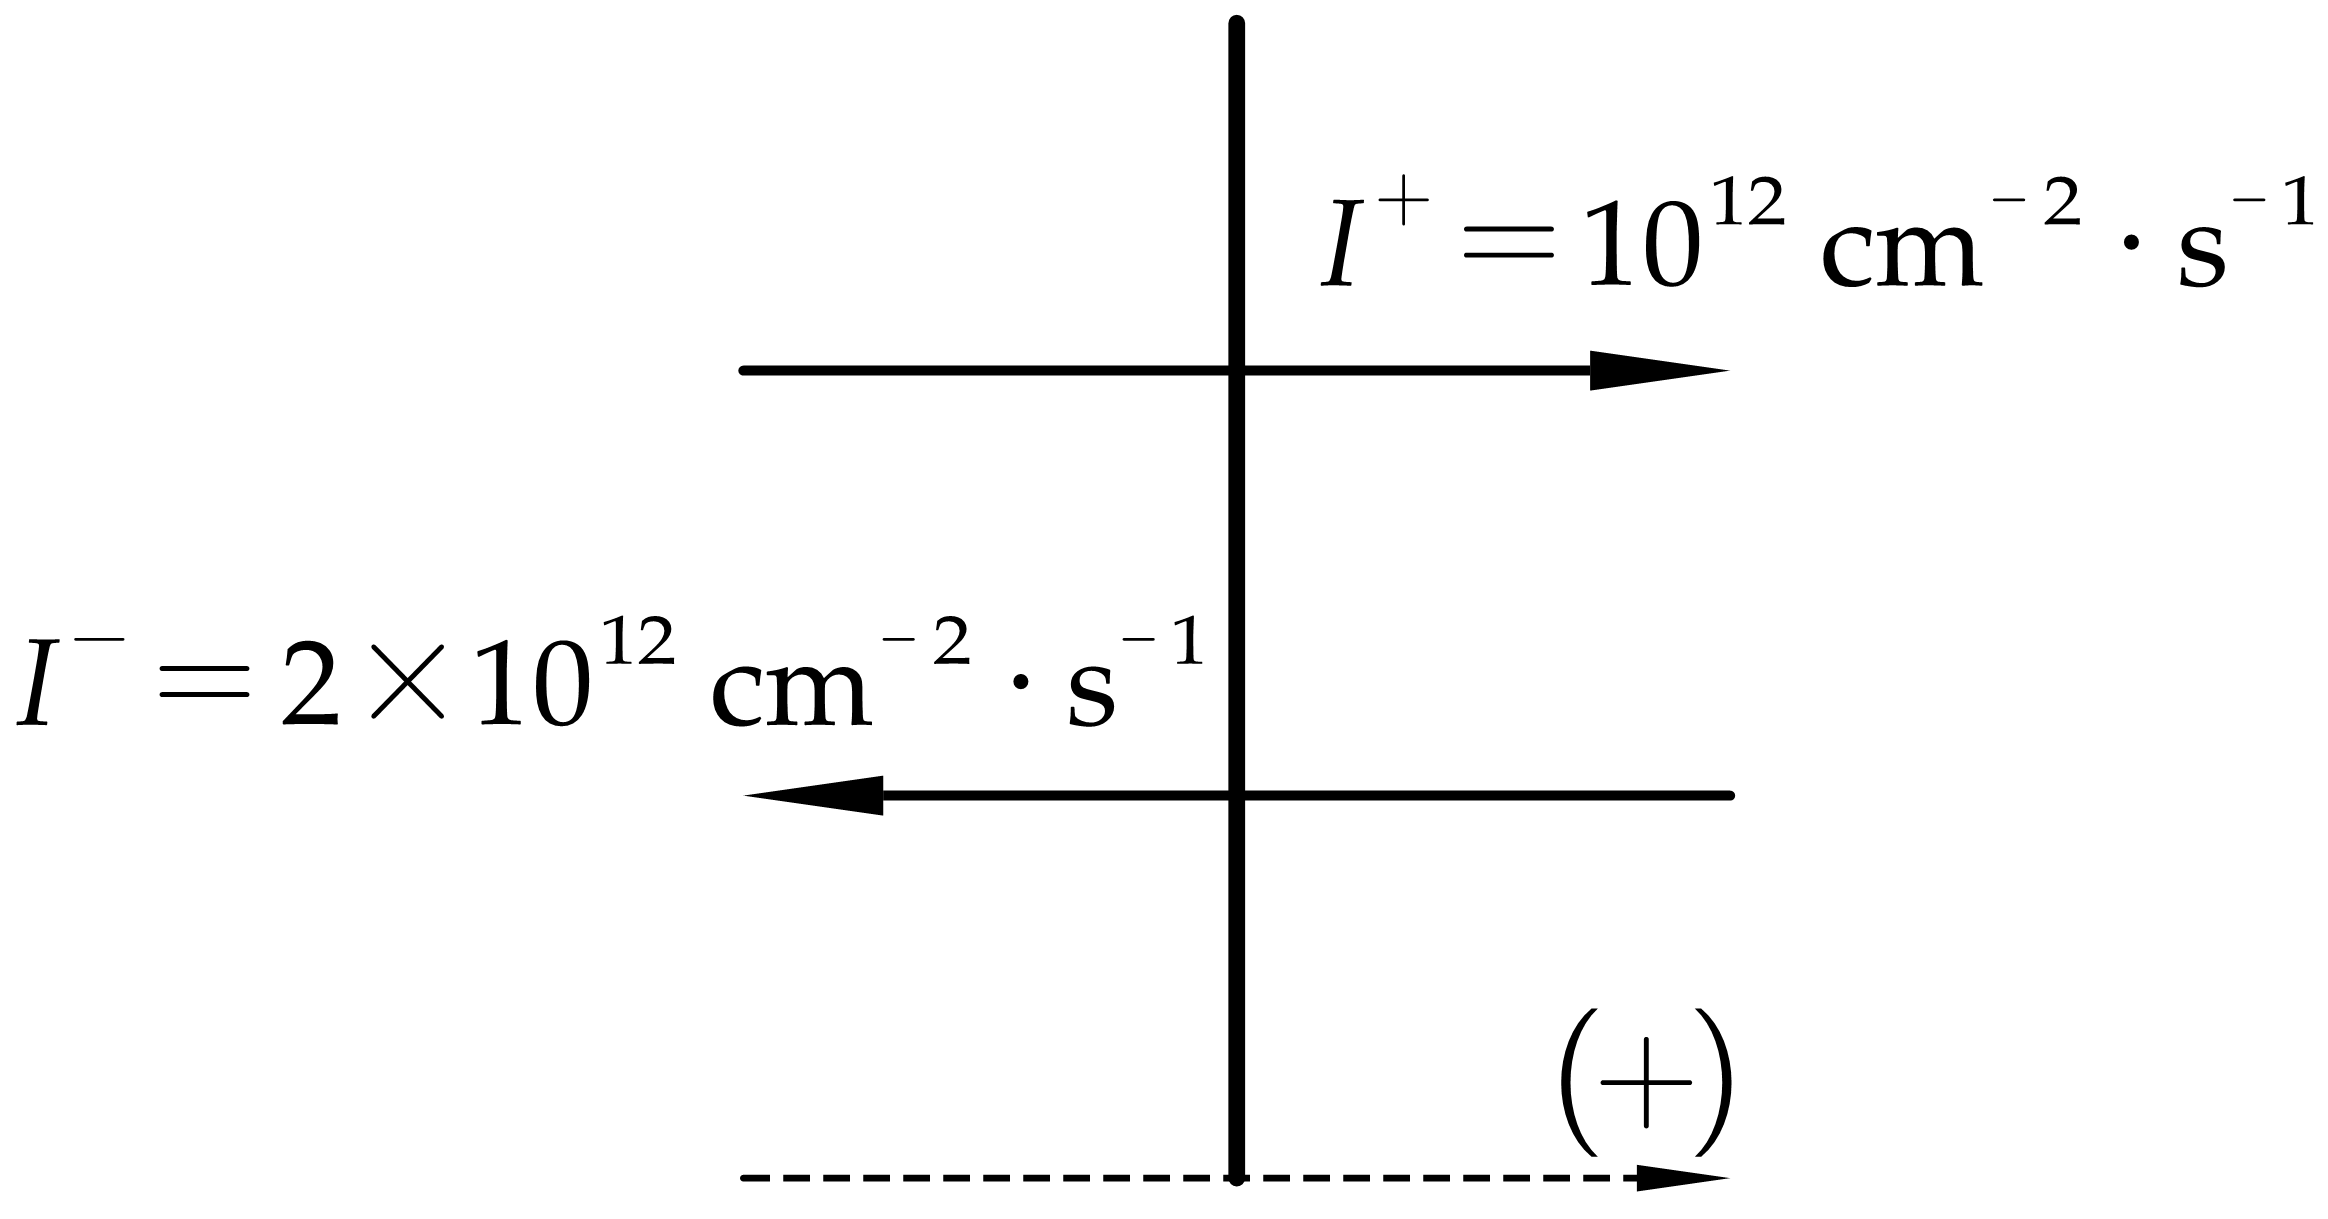
\includegraphics[scale=1.5]{figures/fig4.2.png}
        \end{figure}
        如图所示,取水平向右为正方向,则
        \begin{enumerate}[(1)]
            \item $\phi = I^{+} + I^{-} = 3\times 10^{12}\,\symrm{cm^{-2}\cdot s^{-1}}$;
            \item $J = I^{+} - I^{-} = -10^{12}\,\symrm{cm^{-2}\cdot s^{-1}}$,\,负号表示其方向与正方向相反;
            \item $R_{\symrm{a}} = \vSigma_{\symrm{a}}\phi = 19.2\times 3\times 10^{12}\,\symrm{cm^{-3}\cdot s^{-1}} = 5.76\times 10^{13}\,\symrm{cm^{-3}\cdot s^{-1}}$.
        \end{enumerate}
    \end{solution}
\end{exercise}

\begin{exercise}
    在某球形裸堆($R=0.5\,\symrm{m}$)内中子注量率分布为:
    \begin{equation*}
        \phi(r) = \frac{5\times 10^{13}\,\symrm{cm^{-1}\cdot s^{-1}}}{r} \nsin \left(\frac{\pi r}{R}\right)\,\symrm{cm^{-2}\cdot s^{-1}}
    \end{equation*}
    试求:
    \begin{enumerate}[(1)]
        \item $\phi(0)$;
        \item $J(r)$的表达式,设$D = 0.8\times 10^{-2}\,\symrm{m}$;
        \item 每秒从堆表面泄漏的总中子数(假设外推距离很小可忽略不计)。
    \end{enumerate}
    \begin{solution}
        \begin{enumerate}[(1)]
            \item \begin{equation*}
                \phi = \lim_{r\to 0} \frac{5\times 10^{13}}{r} \nsin \left(\frac{\pi r}{R}\right) = \lim_{r\to 0} \frac{5\times 10^{13}}{r} \cdot \frac{\pi r}{R} = 5\times 10^{13} \times \frac{\pi}{50}\,\symrm{cm^{-2}\cdot s^{-1}} = \pi \times 10^{12}\,\symrm{cm^{-2}\cdot s^{-1}}
            \end{equation*}
            \item \begin{equation*}
                J(r) = -D\nabla \phi(r) = -D \dv{\phi(r)}{r} = 4\times 10^{13} \left[\frac{1}{r^2}\nsin \left(\frac{\pi r}{50}\right) - \frac{\pi}{50 r} \ncos\left(\frac{\pi r}{50}\right)\right]\,\symrm{cm^{-2}\cdot s^{-1}}
            \end{equation*}
            \item \begin{equation*}
                L = J(R)\cdot 4\pi R^2 = 4\times 10^{13} \left[\frac{1}{50^2}\nsin \left(\frac{50 \pi}{50}\right) - \frac{\pi}{50 \times 50} \ncos\left(\frac{50\pi}{50}\right)\right]\times 4\pi\times 50^2 \,\symrm{s^{-1}} = 1.579\times 10^{15}\,\symrm{s^{-1}}
            \end{equation*}
        \end{enumerate}
    \end{solution}
\end{exercise}

\begin{exercise}
    无限纯吸收介质(中子扩散系数为$D$,中子平均自由程为$\lambda$)内,在坐标$(-a,\,0,\,0)$和$(a,\,0,\,0)$处分别有两个源强为$S\,\symrm{s^{-1}}$的点源,试求坐标原点$P_1$和坐标$(0,\,a,\,0)\,P_2$处的中子注量率和中子流密度。
    \begin{solution}
        取$xy$平面,如图所示
        \begin{figure}[H]
            \centering
            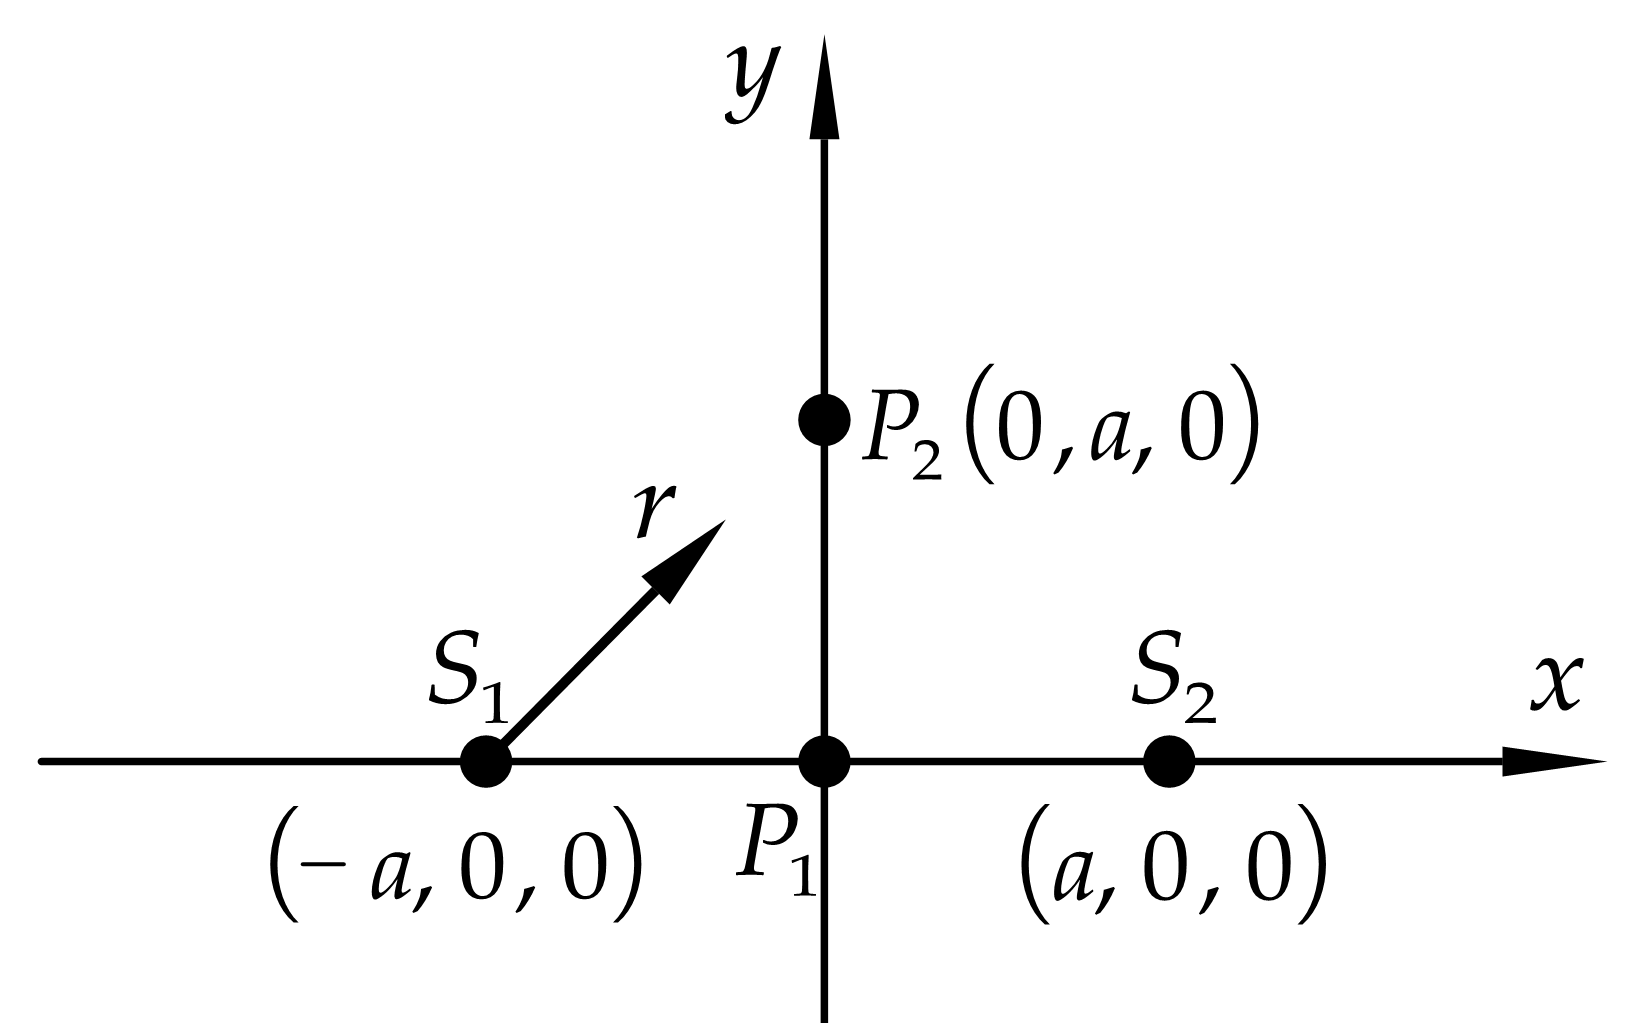
\includegraphics[scale=1.5]{figures/fig4.4.png}
        \end{figure}
        以$S_1$为原点建立一维球坐标系$S_1-r$,则单能中子稳态扩散方程
        \begin{equation*}
            \nabla^2\phi(r)-\frac{\phi(r)}{L^2} = 0,\,r>0
        \end{equation*}
        其中,$r^2 = (x+a)^2+y^2$,$x\neq -a$且$y\neq 0$。

        通解为
        \begin{equation*}
            \phi(r) = A\frac{\symrm{e}^{-r/L}}{r} + C\frac{\symrm{e}^{r/L}}{r}
        \end{equation*}
        边界条件
        \begin{enumerate}[(a)]
            \item $\phi(r)$为有限正值,于是$C=0$;
            \item $\lim\limits_{r\to 0} J(r)\cdot 4\pi r^2 = S$
        \end{enumerate}

        解得
        \begin{align*}
            &J(r) = \frac{S}{4\pi r}\left(\frac{1}{L}+\frac{1}{r}\right)\symrm{e}^{-r/L} = \frac{S}{4\pi r}\left(\frac{1}{L}+\frac{1}{r}\right)\symrm{e}^{-r/\sqrt{D\lambda}} \\
            &\phi(r) = \frac{S\symrm{e}^{-r/L}}{4\pi D r} = \frac{S\symrm{e}^{-r/\sqrt{D\lambda}}}{4\pi D r}
        \end{align*}
        $S_2$与$S_1$源强相等且对称,则
        \begin{enumerate}[(1)]
            \item $P_1$点
            \begin{align*}
                &J_{P_1} = 0 \\
                &\phi_{P_1} = 2\phi(a) = \frac{S\symrm{e}^{-a/\sqrt{D\lambda}}}{2\pi D a}
            \end{align*}
            \item $P_2$点
            \begin{align*}
                &J_{P_2} = \sqrt{2}J(\sqrt{2}a) = \frac{S}{4\pi a}\left(\frac{1}{L}+\frac{1}{\sqrt{2}a}\right)\symrm{e}^{-\sqrt{2}a/\sqrt{D\lambda}} \\
                &\phi_{P_2} = 2\phi(\sqrt{2}a) = \frac{\sqrt{2}S\symrm{e}^{-\sqrt{2}a/\sqrt{D\lambda}}}{4\pi D a}
            \end{align*}
        \end{enumerate}
    \end{solution}
\end{exercise}

\begin{exercise}
    试求边长为$a,\,b,\,c$(包括外推距离)的长方体裸堆的几何曲率和中子注量率分布。设有一边长$a = b = 0.5\,\symrm{m},\,c = 0.6\,\symrm{m}$(包括外推距离)的长方体裸堆,$L = 0.0434\,\symrm{m},\,\tau = 6\,\symrm{cm^2}$。
    \begin{enumerate}[(1)]
        \item 求达到临界时所必需的$K_{\infty}$;
        \item 如果功率为$5000\,\symrm{kW},\,\vSigma_{\symrm{f}} = 4.01\,\symrm{m^{-1}}$,假设每次裂片释放出的能量为$200\,\symrm{MeV}$,求中子注量率分布。
    \end{enumerate}
    \begin{solution}
        以长方体几何中心为坐标原点建立空间直角坐标系$Oxyz$,如图所示
        \begin{figure}[H]
            \centering
            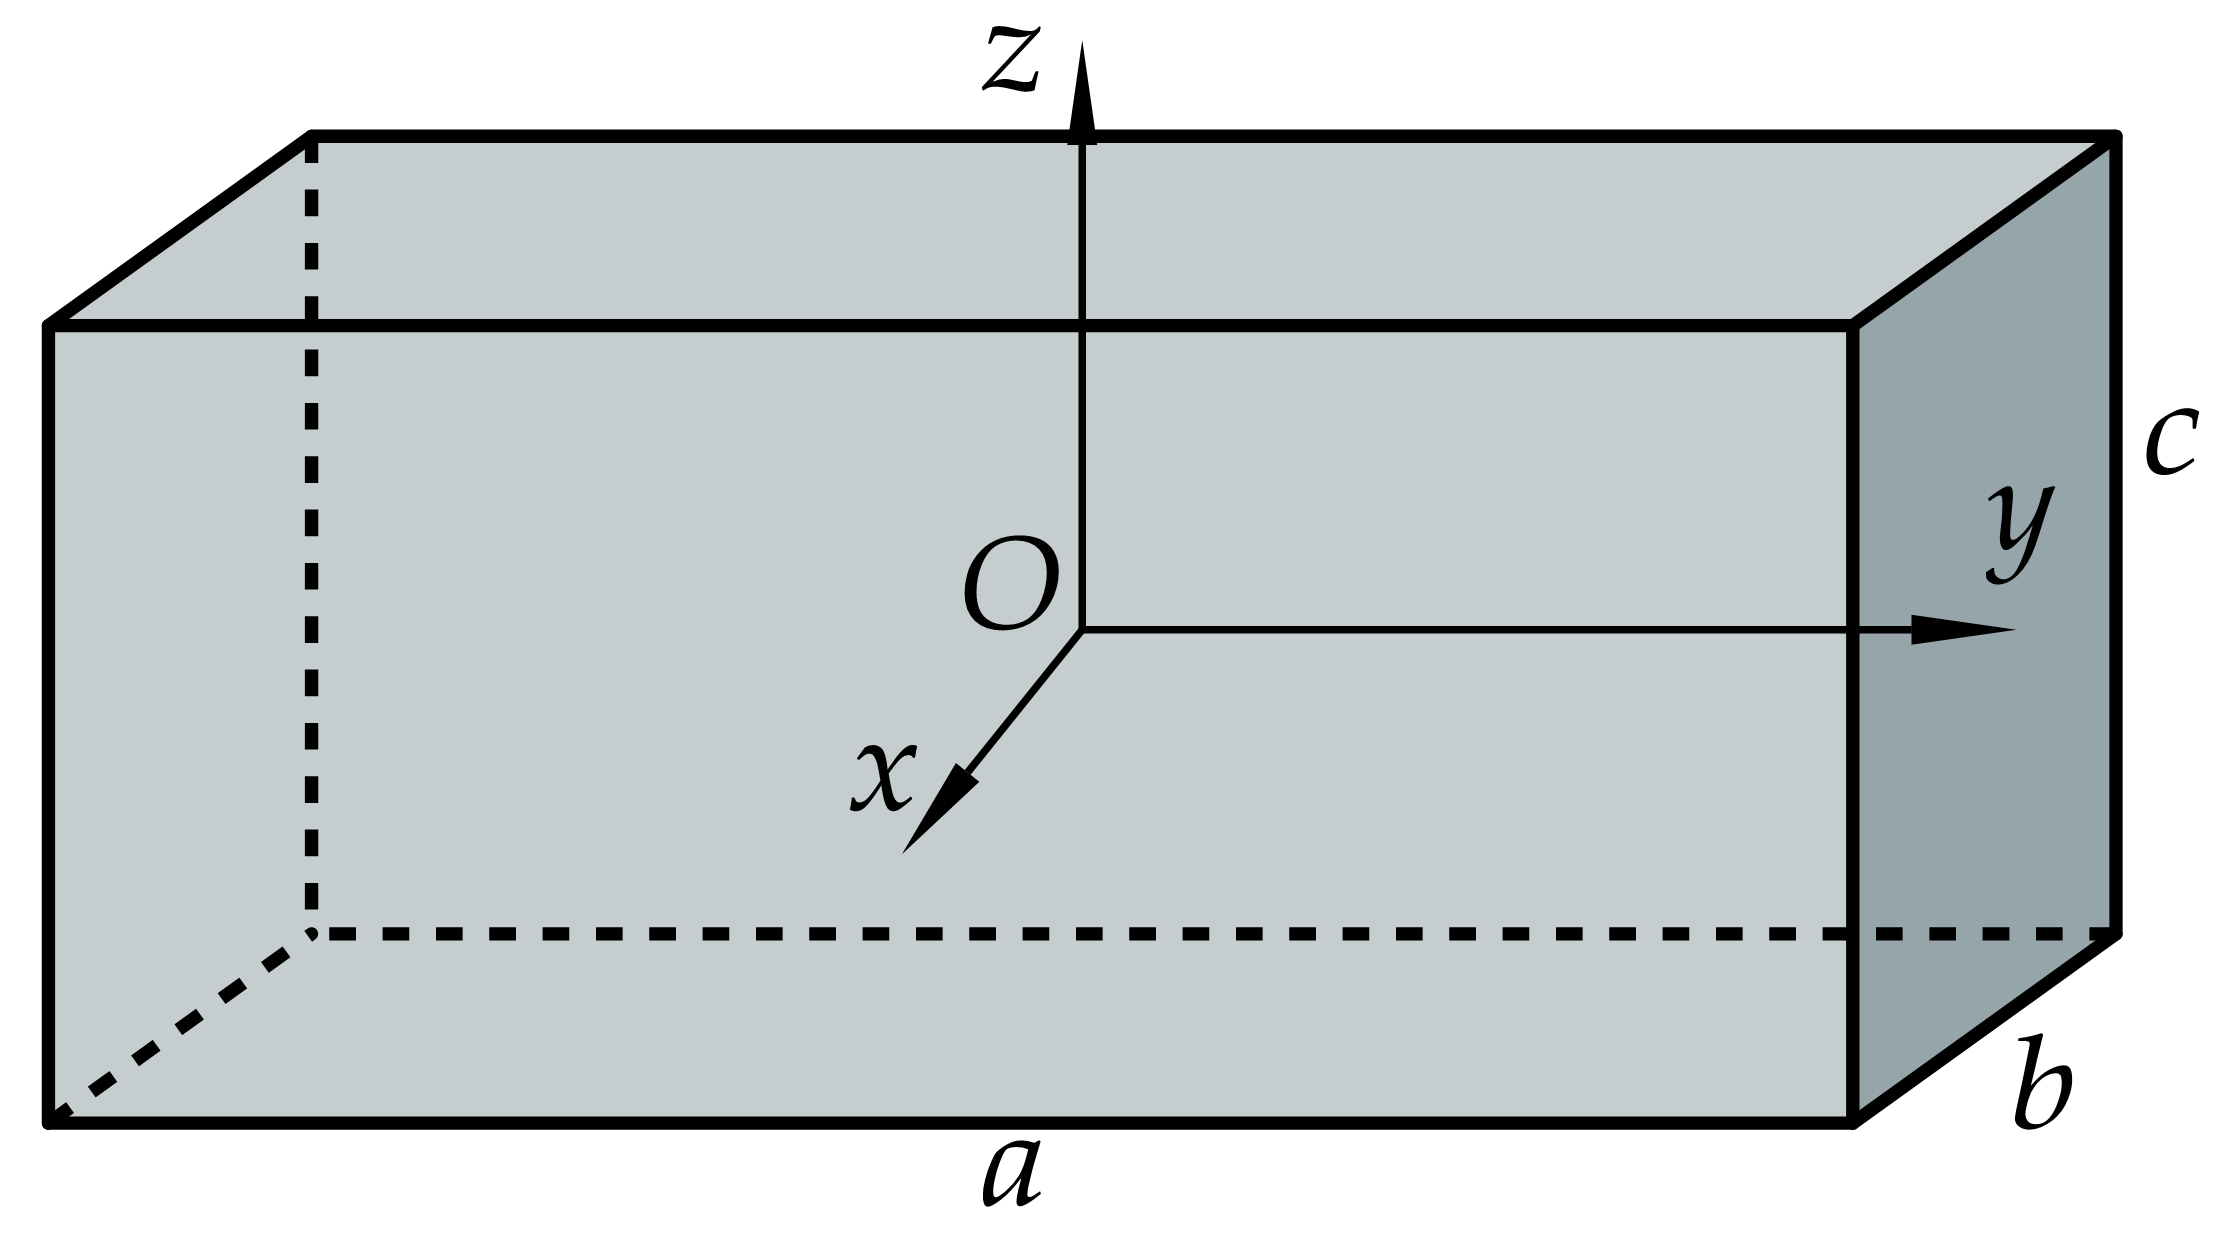
\includegraphics[scale=1]{figures/fig4.5.png}
        \end{figure}
        单能稳态中子扩散方程
        \begin{equation*}
            D\left(\pddv{\phi}{x}+\pddv{\phi}{y}+\pddv{\phi}{z}\right) - \vSigma_{\symrm{a}}\phi + k_{\infty}\vSigma_{\symrm{a}}\phi = 0
        \end{equation*}

        边界条件
        \begin{equation*}
            \phi\left(\pm \frac{a}{2},\,y,\,z\right) = \phi\left(x,\,\pm \frac{b}{2},\,z\right) = \phi\left(x,\,y,\,\pm \frac{c}{2}\right) = 0
        \end{equation*}

        分离变量$\phi(x,\,y,\,z) = \varphi_x(x)\varphi_y(y)\varphi_y(y)$,代入扩散方程,得
        \begin{equation*}
            \frac{\nabla^2\varphi_x(x)}{\varphi_x(x)} + \frac{\nabla^2\varphi_y(y)}{\varphi_y(y)} + \frac{\nabla^2\varphi_z(z)}{\varphi_z(z)} = -\frac{k_{\infty}-1}{L^2}
        \end{equation*}

        令
        \begin{equation*}
            \frac{\nabla^2\varphi_x(x)}{\varphi_x(x)} = -B_x^2 \Rightarrow \nabla^2\varphi_x(x) + B_x^2\varphi_x(x) = 0
        \end{equation*}
        通解为$\varphi_x(x) = A_{nx}\ncos B_{nx}x + C_{nx}\nsin B_{nx}x$。

        \begin{enumerate}[(a)]
            \item 由通量对称分布,得$C_{nx}=0$;
            \item 由边界条件,得$\varphi_x(a/2) = A_{nx}\ncos(aB_{nx}/2) = 0 \Rightarrow B_{nx} = \frac{(2n-1)\pi}{a}\,n=1,\,2,\,3,\,\cdots$.
        \end{enumerate}

        稳态时,取$B_{1x} = \frac{\pi}{a}$,同理,$B_{1y} = \frac{\pi}{b},\,B_{1z} = \frac{\pi}{c}$,\,故几何曲率和中子注量率分布为
        \begin{align*}
            &B_{\symrm{g}}^2 = \left(\frac{\pi}{a}\right)^2 + \left(\frac{\pi}{b}\right)^2 + \left(\frac{\pi}{c}\right)^2 \\
            &\phi = A'_n \ncos\left(\frac{\pi}{a}x\right) \ncos\left(\frac{\pi}{b}y\right) \ncos\left(\frac{\pi}{c}z\right)
        \end{align*}

        \begin{enumerate}[(1)]
            \item 由题意,得几何曲率
            \begin{equation*}
                B_{\symrm{g}}^2 = \left(\frac{\pi}{0.5}\right)^2 + \left(\frac{\pi}{0.5}\right)^2 + \left(\frac{\pi}{0.6}\right)^2\,\symrm{m^{-2}} = 106.4\,\symrm{m^{-2}}
            \end{equation*}
            临界时,满足
            \begin{equation*}
                \frac{k_{\infty} - 1}{M^2} = B_{\symrm{g}}^2 \Rightarrow k_{\infty} = B_{\symrm{g}}^2(L^2+\tau) + 1 = 106.4 \times (0.0434^2 + 0.0006) + 1 = 1.264
            \end{equation*}
            \item 由题意,有
            \begin{equation*}
                P = E_{\symrm{f}}\int_V \vSigma_{\symrm{f}} \phi \dd{V} = E_{\symrm{f}} \vSigma_{\symrm{f}} A_n \int_{-a/2}^{a/2} \ncos\left(\frac{\pi}{a}x\right) \dd{x} \int_{-b/2}^{b/2} \ncos\left(\frac{\pi}{b}y\right) \dd{y} \int_{-c/2}^{c/2} \ncos\left(\frac{\pi}{c}z\right) \dd{z} = E_{\symrm{f}} \vSigma_{\symrm{f}} A_n abc \left(\frac{2}{\pi}\right)^3
            \end{equation*}
            于是
            \begin{equation*}
                A_n = \frac{P(\pi/2)^3}{E_{\symrm{f}} \vSigma_{\symrm{f}} abc} = \frac{5\times 10^6 \times (\pi/2)^3}{200 \times 10^6 \times 1.6 \times 10^{-19} \times 4.01 \times 0.5 \times 0.5 \times 0.6}\,\symrm{m^{-2}\cdot s^{-1}} = 1.007 \times 10^{18}\,\symrm{m^{-2}\cdot s^{-1}}
            \end{equation*}
            故中子注量率分布
            \begin{equation*}
                \phi(x,\,y,\,z) = 1.007 \times 10^{18} \ncos\left(2\pi x\right) \ncos\left(2\pi y\right) \ncos\left(\frac{5\pi}{3}z\right)\,\symrm{m^{-2}\cdot s^{-1}}
            \end{equation*}
        \end{enumerate}
    \end{solution}
\end{exercise}

\begin{exercise}
    设一座重水-铀核反应堆堆芯的$k_{\infty} = 1.28,\,L^2 = 1.8\times 10^{-2}\,\symrm{m^2},\,\tau = 1.20\times 10^{-2}\,\symrm{m^2}$。试按单群理论,修正单群理论的临界方程分别求出该堆芯的材料曲率和达到临界时总的中子不泄漏概率。
    \begin{solution}
        \begin{enumerate}[(1)]
            \item 按单群理论
            \begin{align*}
                &B_{\symrm{m}}^2 = \frac{k_{\infty} - 1}{L^2} = \frac{1.28 - 1}{1.8\times 10^{-2}}\,\symrm{m^{-2}} = 15.56\,\symrm{m^{-2}} \\
                &P_L = \frac{1}{L^2 B_{\symrm{g}}^2} = \frac{1}{L^2 B_{\symrm{m}}^2} = \frac{1}{1 + 1.8\times 10^{-2}\times 15.56} = 0.7812
            \end{align*}
            \item 按修正单群理论
            \begin{align*}
                &B_{\symrm{m}}^2 = \frac{k_{\infty} - 1}{M^2} = \frac{k_{\infty} - 1}{L^2 + \tau} = \frac{1.28 - 1}{1.8\times 10^{-2} + 1.2\times 10^{-2}}\,\symrm{m^{-2}} = 9.333\,\symrm{m^{-2}} \\
                &P_L = \frac{1}{M^2 B_{\symrm{g}}^2} = \frac{1}{(L^2 + \tau) B_{\symrm{m}}^2} = \frac{1}{1 + (1.8\times 10^{-2} + 1.2\times 10^{-2})\times 9.333} = 0.7813
            \end{align*}
        \end{enumerate}
    \end{solution}
\end{exercise}

\begin{exercise}
    设有圆柱形铀一水栅格装置,$R = 0.50\,\symrm{m}$,水位高度$H = 1.0\,\symrm{m}$,设栅格参数为:$k_{\infty} = 1.19,\,L^2 = 6.6\times 10^{-4}\,\symrm{m^2},\,\tau = 0.50\times 10^{-2}\,\symrm{m^2}$。
    \begin{enumerate}[(1)]
        \item 试求该装置的有效增殖因数$\keff$;
        \item 当该装置恰好达到临界时,水位高度$H$等于多少?
        \item 设某压水堆以该铀-水栅格作为芯部,堆芯的尺寸为$R = 1.66\,\symrm{m},\,H = 3.5\,\symrm{m}$,若反射层节省估算为$\delta_{\symrm{r}} = 0.07\,\symrm{m},\,\delta_{\symrm{H}} = 0.1\,\symrm{m}$,试求核反应堆的初始反应性$\rho_0$。
    \end{enumerate}
    \begin{solution}
        假设$R=0.5\,\symrm{m},\,H=1.0\,\symrm{m}$已包含外推距离。
        \begin{enumerate}[(1)]
            \item 几何曲率
            \begin{equation*}
                B_{\symrm{g}}^2 = \left(\frac{2.405}{R}\right)^2 + \left(\frac{\pi}{H}\right)^2 = \left(\frac{2.405}{0.5}\right)^2 + \left(\frac{\pi}{1}\right)^2\,\symrm{m^{-2}} = 33.01\,\symrm{m^{-2}}
            \end{equation*}
            有效增殖因数
            \begin{equation*}
                \keff = \frac{k_{\infty}}{1 + M^2 B_{\symrm{g}}^2} = \frac{k_{\infty}}{1 + (L^2 + \tau) B_{\symrm{g}}^2} = \frac{1.19}{1 + (6.6\times 10^{-4} + 0.5\times 10^{-2}) \times 33.01} = 1.003
            \end{equation*}
            \item 材料曲率
            \begin{equation*}
                B_{\symrm{m}}^2 = \frac{k_{\infty} - 1}{M^2} = \frac{k_{\infty} - 1}{L^2 + \tau} = \frac{1.19 - 1}{6.6\times 10^{-4} + 0.5\times 10^{-2}}\,\symrm{m^{-2}} = 33.57\,\symrm{-2}
            \end{equation*}
            临界时,有
            \begin{equation*}
                B_{\symrm{g}}^2 = \left(\frac{2.405}{R}\right)^2 + \left(\frac{\pi}{H}\right)^2 = B_{\symrm{m}}^2 = 33.57\,\symrm{-2}
            \end{equation*}
            
            由此解得$H = 0.9726\,\symrm{m}$.
            \item 等效裸堆尺寸
            \begin{equation*}
                \begin{cases}
                    R_{\symrm{eff}} = R + \delta_{\symrm{r}} = 1.66 + 0.07\,\symrm{m} = 1.73\,\symrm{m} \\
                    H_{\symrm{eff}} = H + 2\delta_{\symrm{H}} = 3.5 + 2 \times 0.1 = 3.7\,\symrm{m}
                \end{cases}
            \end{equation*}
            几何曲率
            \begin{equation*}
                B_{\symrm{g}}^2 = \left(\frac{2.405}{R_{\symrm{eff}}}\right)^2 + \left(\frac{\pi}{H_{\symrm{eff}}}\right)^2 = \left(\frac{2.405}{1.73}\right)^2 + \left(\frac{\pi}{3.7}\right)^2\,\symrm{m^{-2}} = 2.654\,\symrm{m^{-2}}
            \end{equation*}
            有效增殖因数
            \begin{equation*}
                \keff = \frac{k_{\infty}}{1 + M^2 B_{\symrm{g}}^2} = \frac{k_{\infty}}{1 + (L^2 + \tau) B_{\symrm{g}}^2} = \frac{1.19}{1 + (6.6\times 10^{-4} + 0.5\times 10^{-2}) \times 2.654} = 1.172
            \end{equation*}
            初始反应性
            \begin{equation*}
                \rho_0 = \frac{\keff - 1}{\keff} = \frac{1.172 - 1}{1.172} = 0.1468
            \end{equation*}
        \end{enumerate}
    \end{solution}
\end{exercise}

\begin{exercise}
    一球壳形核反应堆,内半径为$R_1$,外半径为$R_2$(包含外推距离),如果球的内外均为真空,求证单群理论的临界条件为:
    \begin{equation*}
        \ntan BR_2 = \frac{\ntan BR_1 - BR_1}{BR_1\ntan BR_1 + 1}
    \end{equation*}
    \begin{solution}
        \begin{figure}[H]
            \centering
            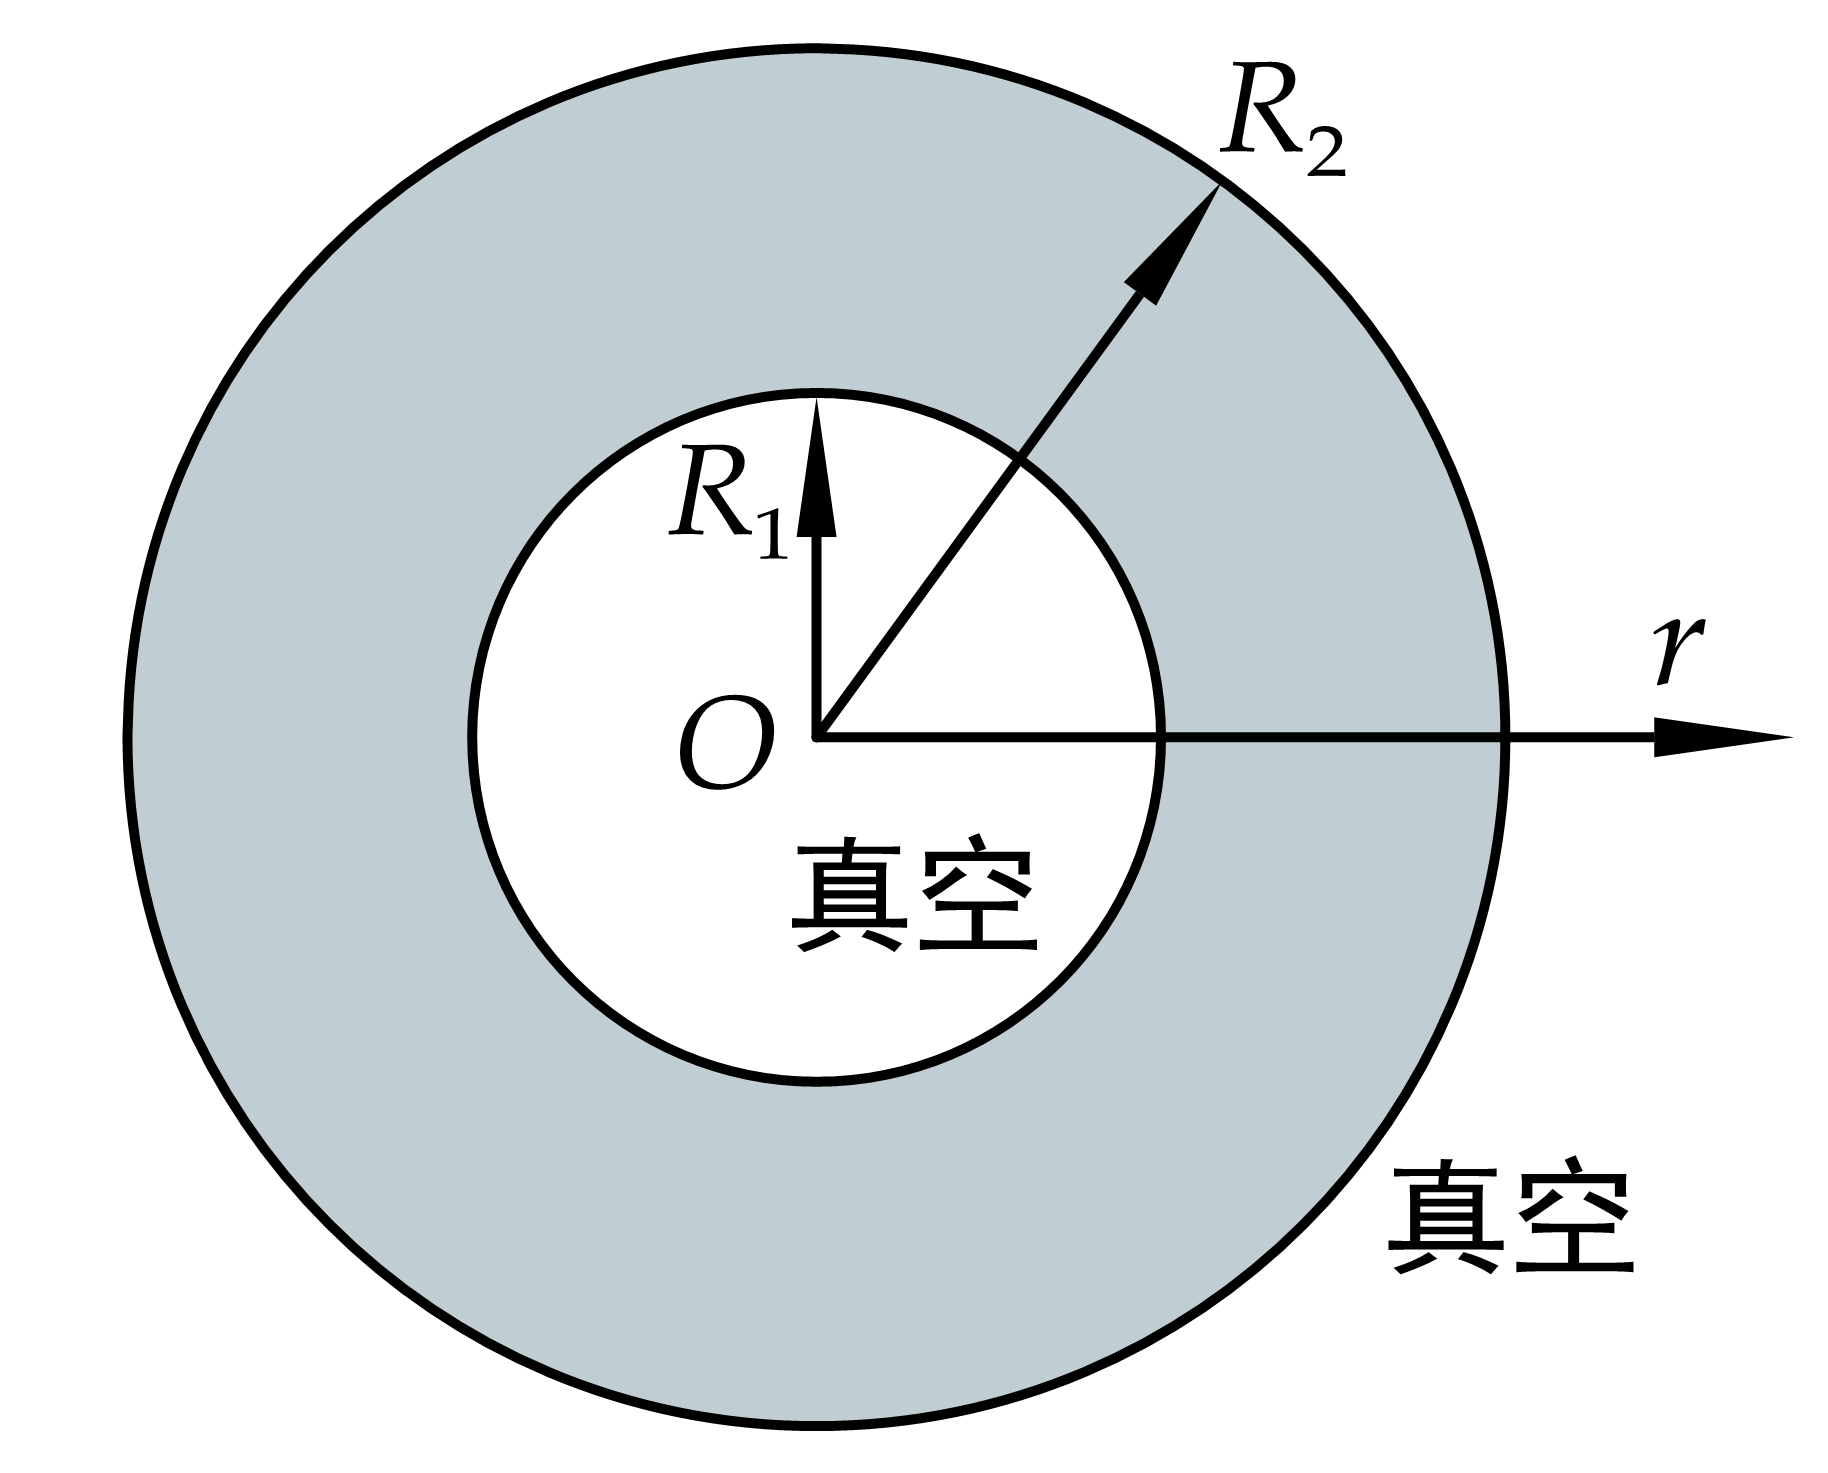
\includegraphics[scale=1]{figures/fig4.8.png}
        \end{figure}
        以球心为坐标原点建立一维球坐标系,如图所示,则临界时单能中子稳态扩散方程(增殖)为
        \begin{equation*}
            \ddv{\phi(r)}{r} + \frac{2}{r} \dv{\phi(r)}{r} + \frac{k_{\infty} - 1}{L^2}\phi(r) = 0 \xrightarrow{B^2 = (k_{\infty} - 1)/L^2} \ddv{\phi(r)}{r} + \frac{2}{r} \dv{\phi(r)}{r} + B^2 \phi(r) = 0
        \end{equation*}
        通解为
        \begin{equation*}
            \phi(r) = A\frac{\nsin Br}{r} + C\frac{\ncos Br}{r}
        \end{equation*}
        
        边界条件
        \begin{enumerate}[(1)]
            \item $\lim\limits_{r\to R_1} J = 0$
            \begin{equation*}
                \lim_{r\to R_1} J = \lim_{r\to R_1} -D\dv{\phi(r)}{r} = \lim_{r\to R_1} -D\left(AB\frac{\ncos Br}{r} - A\frac{\nsin Br}{r^2} - BC\frac{\nsin Br}{r} - C\frac{\ncos Br}{r^2}\right) = 0
            \end{equation*}
            而$D \neq 0$,立即推
            \begin{equation*}
                AB\frac{\ncos BR_1}{R_1} - A\frac{\nsin BR_1}{R_1^2} - BC\frac{\nsin BR_1}{R_1} - C\frac{\ncos BR_1}{R_1^2} = 0
            \end{equation*}
            解得
            \begin{equation*}
                C = A\frac{BR_1 - \ntan BR_1}{BR_1 \ntan BR_1 + 1}
            \end{equation*}
            \item $\phi(R_2) = 0$
            \begin{equation*}
                \phi(R_2) = A\frac{\nsin BR_2}{R_2} + C\frac{\ncos BR_2}{R_2} = 0 \Rightarrow C = -A\ntan BR_2
            \end{equation*}
        \end{enumerate}
        联立可得
        \begin{equation*}
            \ntan BR_2 = \frac{\ntan BR_1 - BR_1}{BR_1\ntan BR_1 + 1}
        \end{equation*}
    \end{solution}
\end{exercise}

\begin{exercise}
    一维无限平板几何下,坐标原点左侧和右侧分别为两种非增殖但含中子源的材料,两种材料的扩散系数相同、中子扩散长度的倒数分别为$\kappa_{\symrm{l}}^2$和$\kappa_{\symrm{r}}^2$,相应的中子源强分别为$\kappa_{\symrm{l}}^2 \vPhi_{\symrm{l}}$和$\kappa_{\symrm{r}}^2 \vPhi_{\symrm{r}}$。
    \begin{enumerate}[(1)]
        \item 试计算该一维无限平板内的中子注量率分布和原点处的中子注量率;
        \item 试画出区间$[-5/\kappa_{\symrm{l}},\,5/\kappa_{\symrm{r}}]$内在$\vPhi_{\symrm{l}}=0,\,\vPhi_{\symrm{r}}=1,\,\kappa_{\symrm{l}}=\kappa_{\symrm{r}}=\kappa$时的中子注量率分布;
        \item 试画出区间$[-5/\kappa_{\symrm{l}},\,5/\kappa_{\symrm{r}}]$内在$\vPhi_{\symrm{l}}=2,\,\vPhi_{\symrm{r}}=1,\,\kappa_{\symrm{l}}=3\kappa,\,\kappa_{\symrm{r}}=\kappa$时的中子注量率分布。
    \end{enumerate}
    \begin{solution}
        \begin{enumerate}[(1)]
            \item 如图所示,以$x>0$为例,有
            \begin{figure}[H]
                \centering
                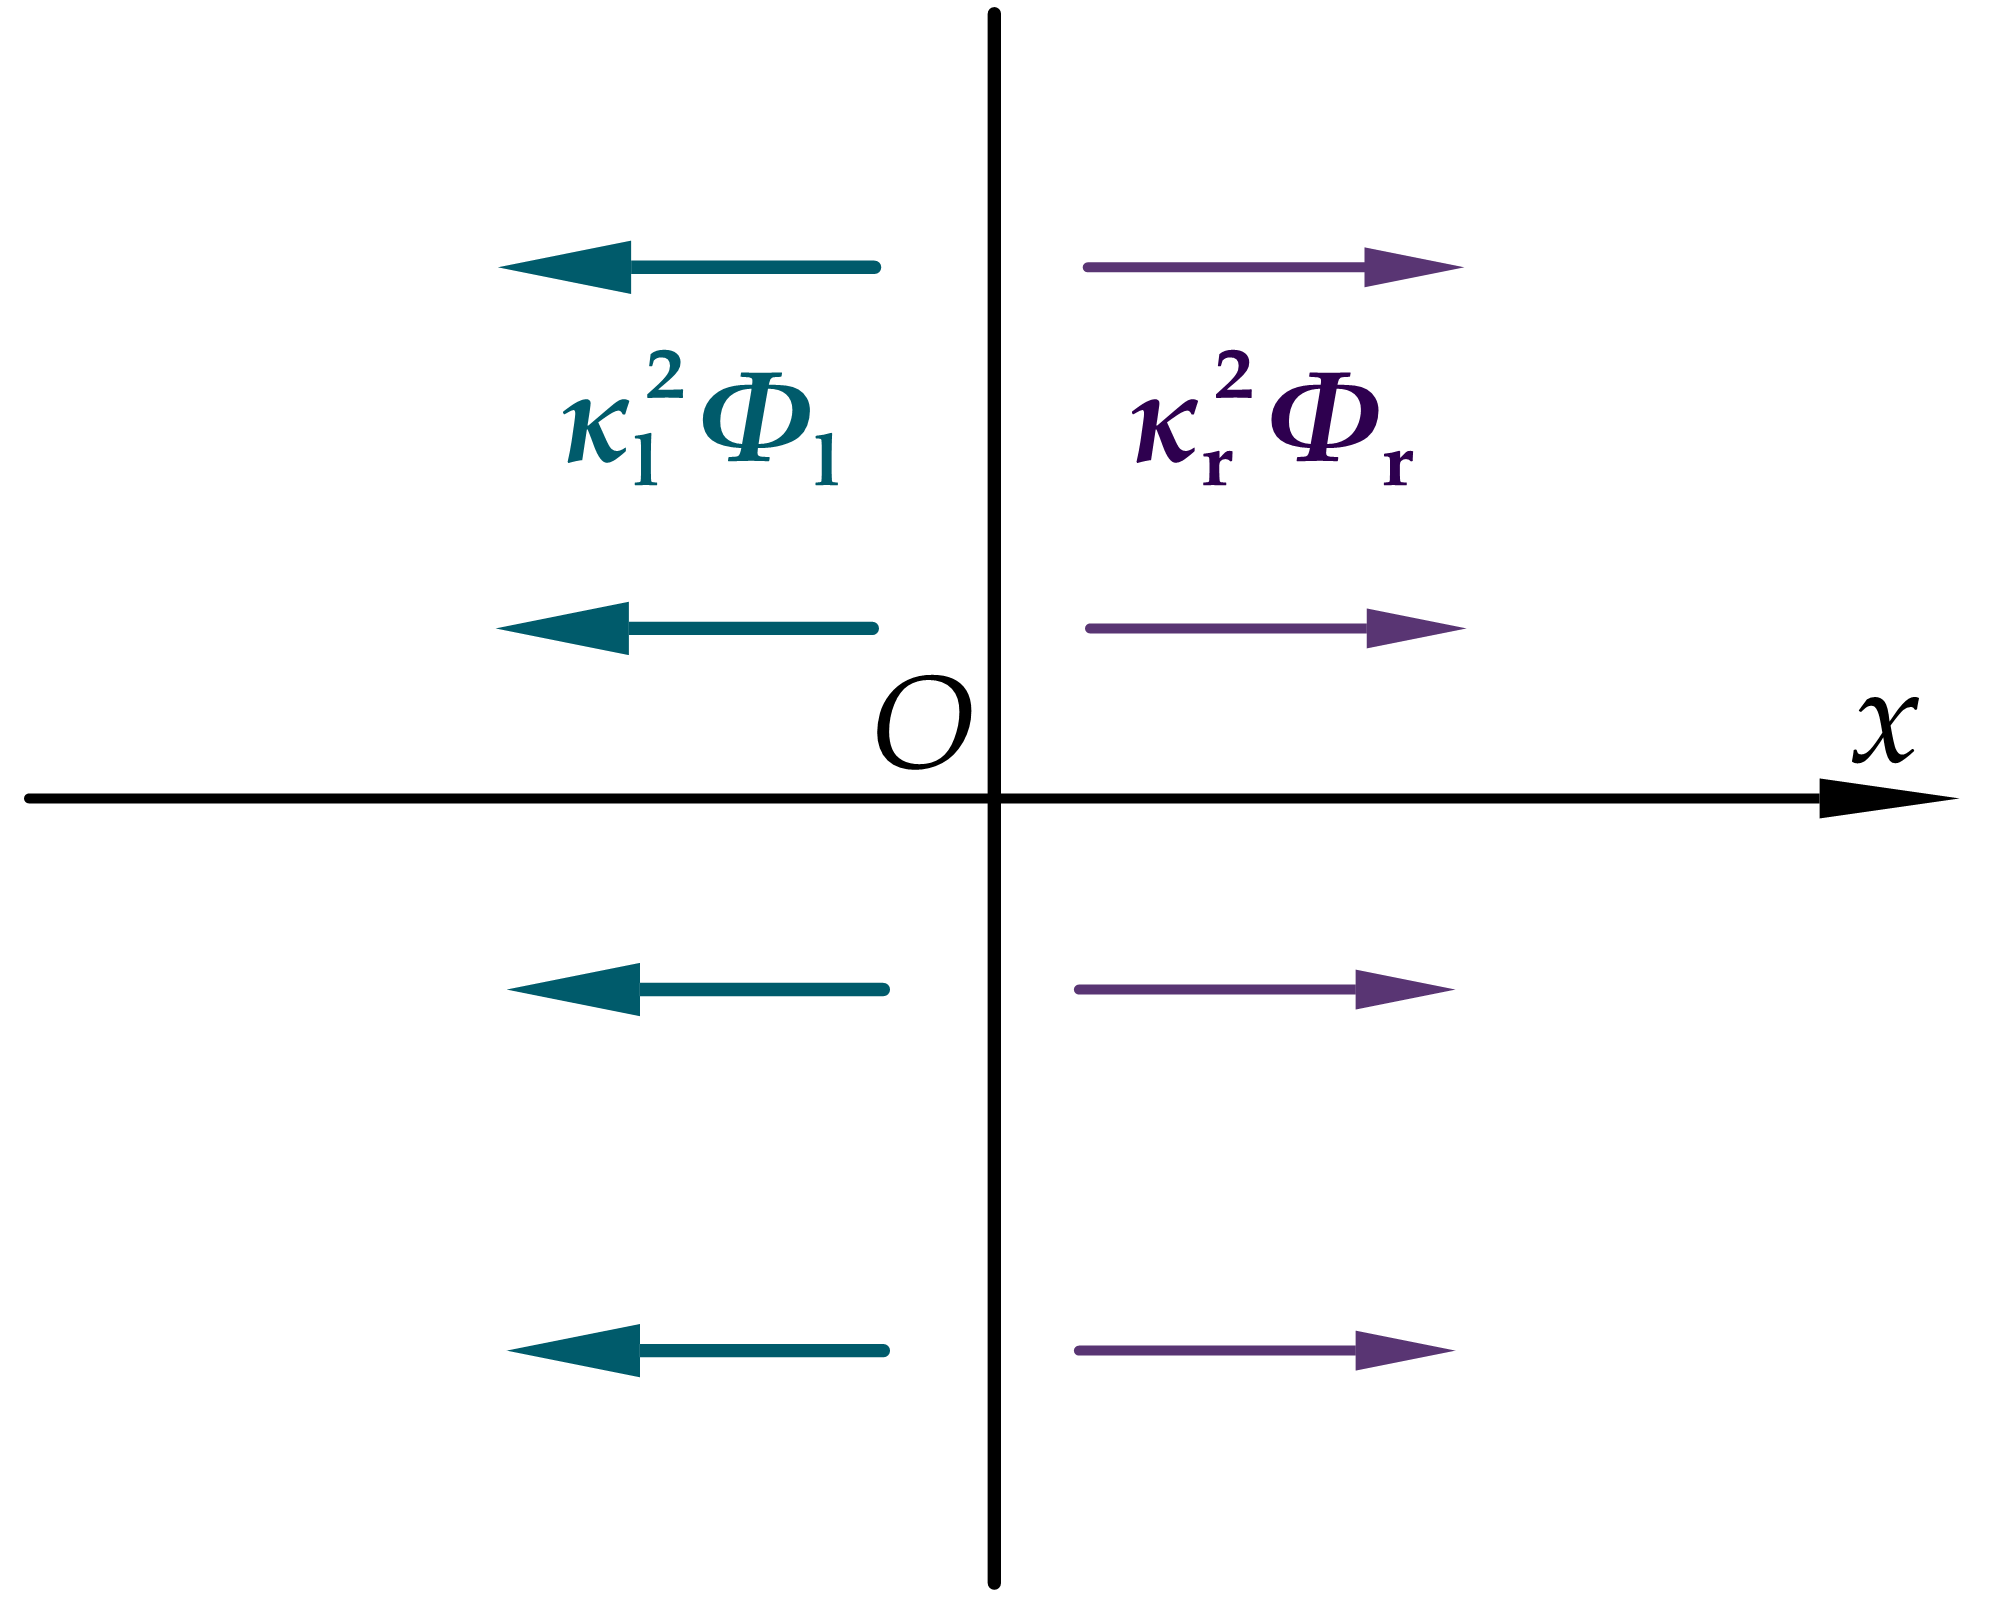
\includegraphics[scale=1]{figures/fig4.9.png}
            \end{figure}
            \begin{equation*}
                \ddv{\phi_{\symrm{r}}(x)}{x} - \frac{\phi_{\symrm{r}}(x)}{L^2} = 0,\,x > 0
            \end{equation*}
            通解为
            \begin{equation*}
                \phi_{\symrm{r}}(x) = A_{\symrm{r}} \symrm{e}^{-x/L_r} + C_{\symrm{r}} \symrm{e}^{x/L_r}
            \end{equation*}
            边界条件
            \begin{enumerate}[(a)]
                \item $\phi_{\symrm{r}}(x)$为有限正值,于是$C_{\symrm{r}} = 0$;
                \item $\lim\limits_{r\to 0^{+}} J_{\symrm{r}}(x) = \kappa_{\symrm{r}}^2 \vPhi_{\symrm{r}} \Rightarrow A_{\symrm{r}} = \frac{\kappa_{\symrm{r}}^2 \vPhi_{\symrm{r}} L_{\symrm{r}}}{D} \xlongequal[\kappa_{\symrm{r}}^2 L_{\symrm{r}}^2 = 1]{\kappa_{\symrm{r}} L_{\symrm{r}} = 1} \frac{\kappa_{\symrm{r}} \vPhi_{\symrm{r}}}{D}$
            \end{enumerate}
            于是
            \begin{equation*}
                \phi_{\symrm{r}}(x) = \frac{\kappa_{\symrm{r}} \vPhi_{\symrm{r}}}{D} \symrm{e}^{-\kappa_{\symrm{r}}x},\,x\geqslant 0
            \end{equation*}
            同理
            \begin{equation*}
                \phi_{\symrm{l}}(x) = \frac{\kappa_{\symrm{l}} \vPhi_{\symrm{l}}}{D} \symrm{e}^{\kappa_{\symrm{l}}x},\,x < 0
            \end{equation*}
            即
            \begin{equation*}
                \phi(x) = \begin{cases}
                    \frac{\kappa_{\symrm{l}} \vPhi_{\symrm{l}}}{D} \symrm{e}^{\kappa_{\symrm{l}}x},\,x < 0 \\
                    \frac{\kappa_{\symrm{r}} \vPhi_{\symrm{r}}}{D} \symrm{e}^{-\kappa_{\symrm{r}}x},\,x > 0
                \end{cases}
            \end{equation*}
            原点处中子注量率不连续,有
            \begin{align*}
                &\phi(0^{-}) = \lim_{x \to 0} \phi_{\symrm{l}}(x) = \lim_{x \to 0} \frac{\kappa_{\symrm{l}} \vPhi_{\symrm{l}}}{D} \symrm{e}^{\kappa_{\symrm{l}}x} = \frac{\kappa_{\symrm{l}} \vPhi_{\symrm{l}}}{D} \\
                &\phi(0^{+}) = \lim_{x \to 0} \phi_{\symrm{r}}(x) = \lim_{x \to 0} \frac{\kappa_{\symrm{r}} \vPhi_{\symrm{r}}}{D} \symrm{e}^{-\kappa_{\symrm{r}}x} = \frac{\kappa_{\symrm{r}} \vPhi_{\symrm{r}}}{D}
            \end{align*}
            \item 由题意,此时
            \begin{equation*}
                \phi(x) = \begin{cases}
                    \phi_{\symrm{l}}(x) = 0,\,x < 0 \\
                    \phi_{\symrm{r}}(x) = \frac{\kappa}{D} \symrm{e}^{-\kappa x},\,x > 0
                \end{cases}
            \end{equation*}
            \begin{figure}[H]
                \centering
                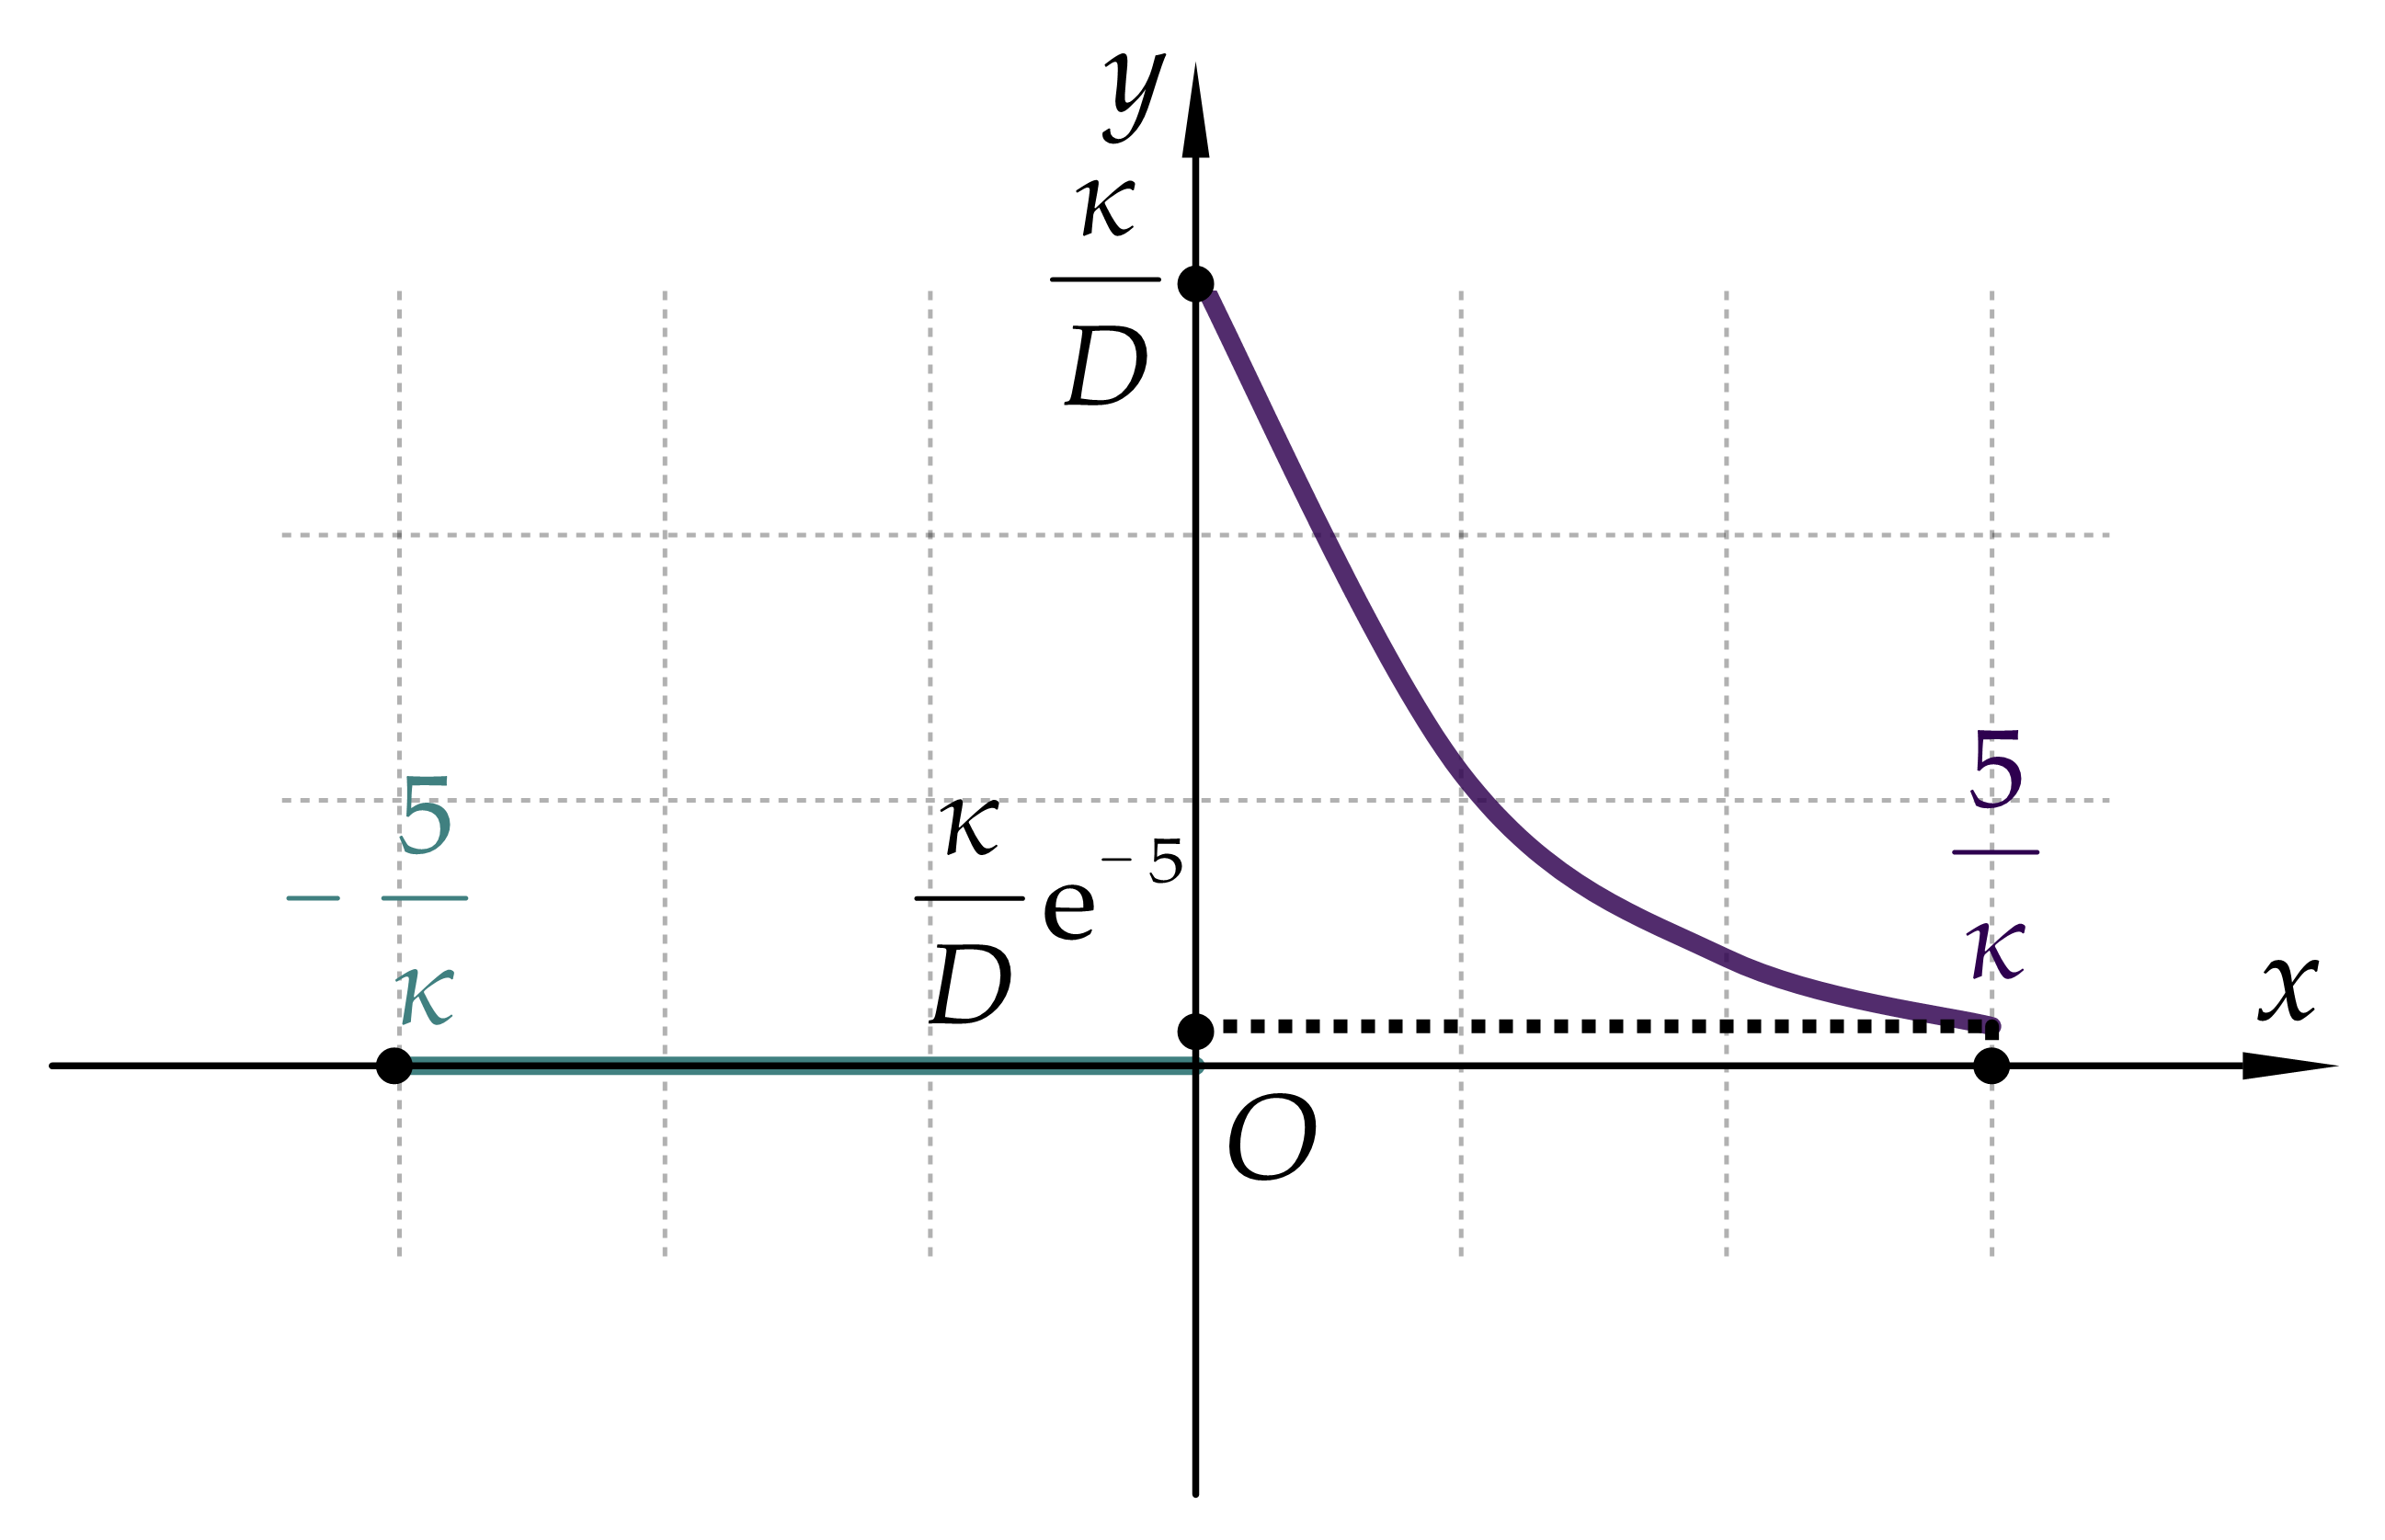
\includegraphics[scale=1]{figures/fig4.9-2.png}
            \end{figure}
            \item 由题意,此时
            \begin{equation*}
                \phi(x) = \begin{cases}
                    \phi_{\symrm{l}}(x) = \frac{6\kappa}{D} \symrm{e}^{3\kappa x},\,x < 0 \\
                    \phi_{\symrm{r}}(x) = \frac{\kappa}{D} \symrm{e}^{-\kappa x},\,x > 0
                \end{cases}
            \end{equation*}
            \begin{figure}[H]
                \centering
                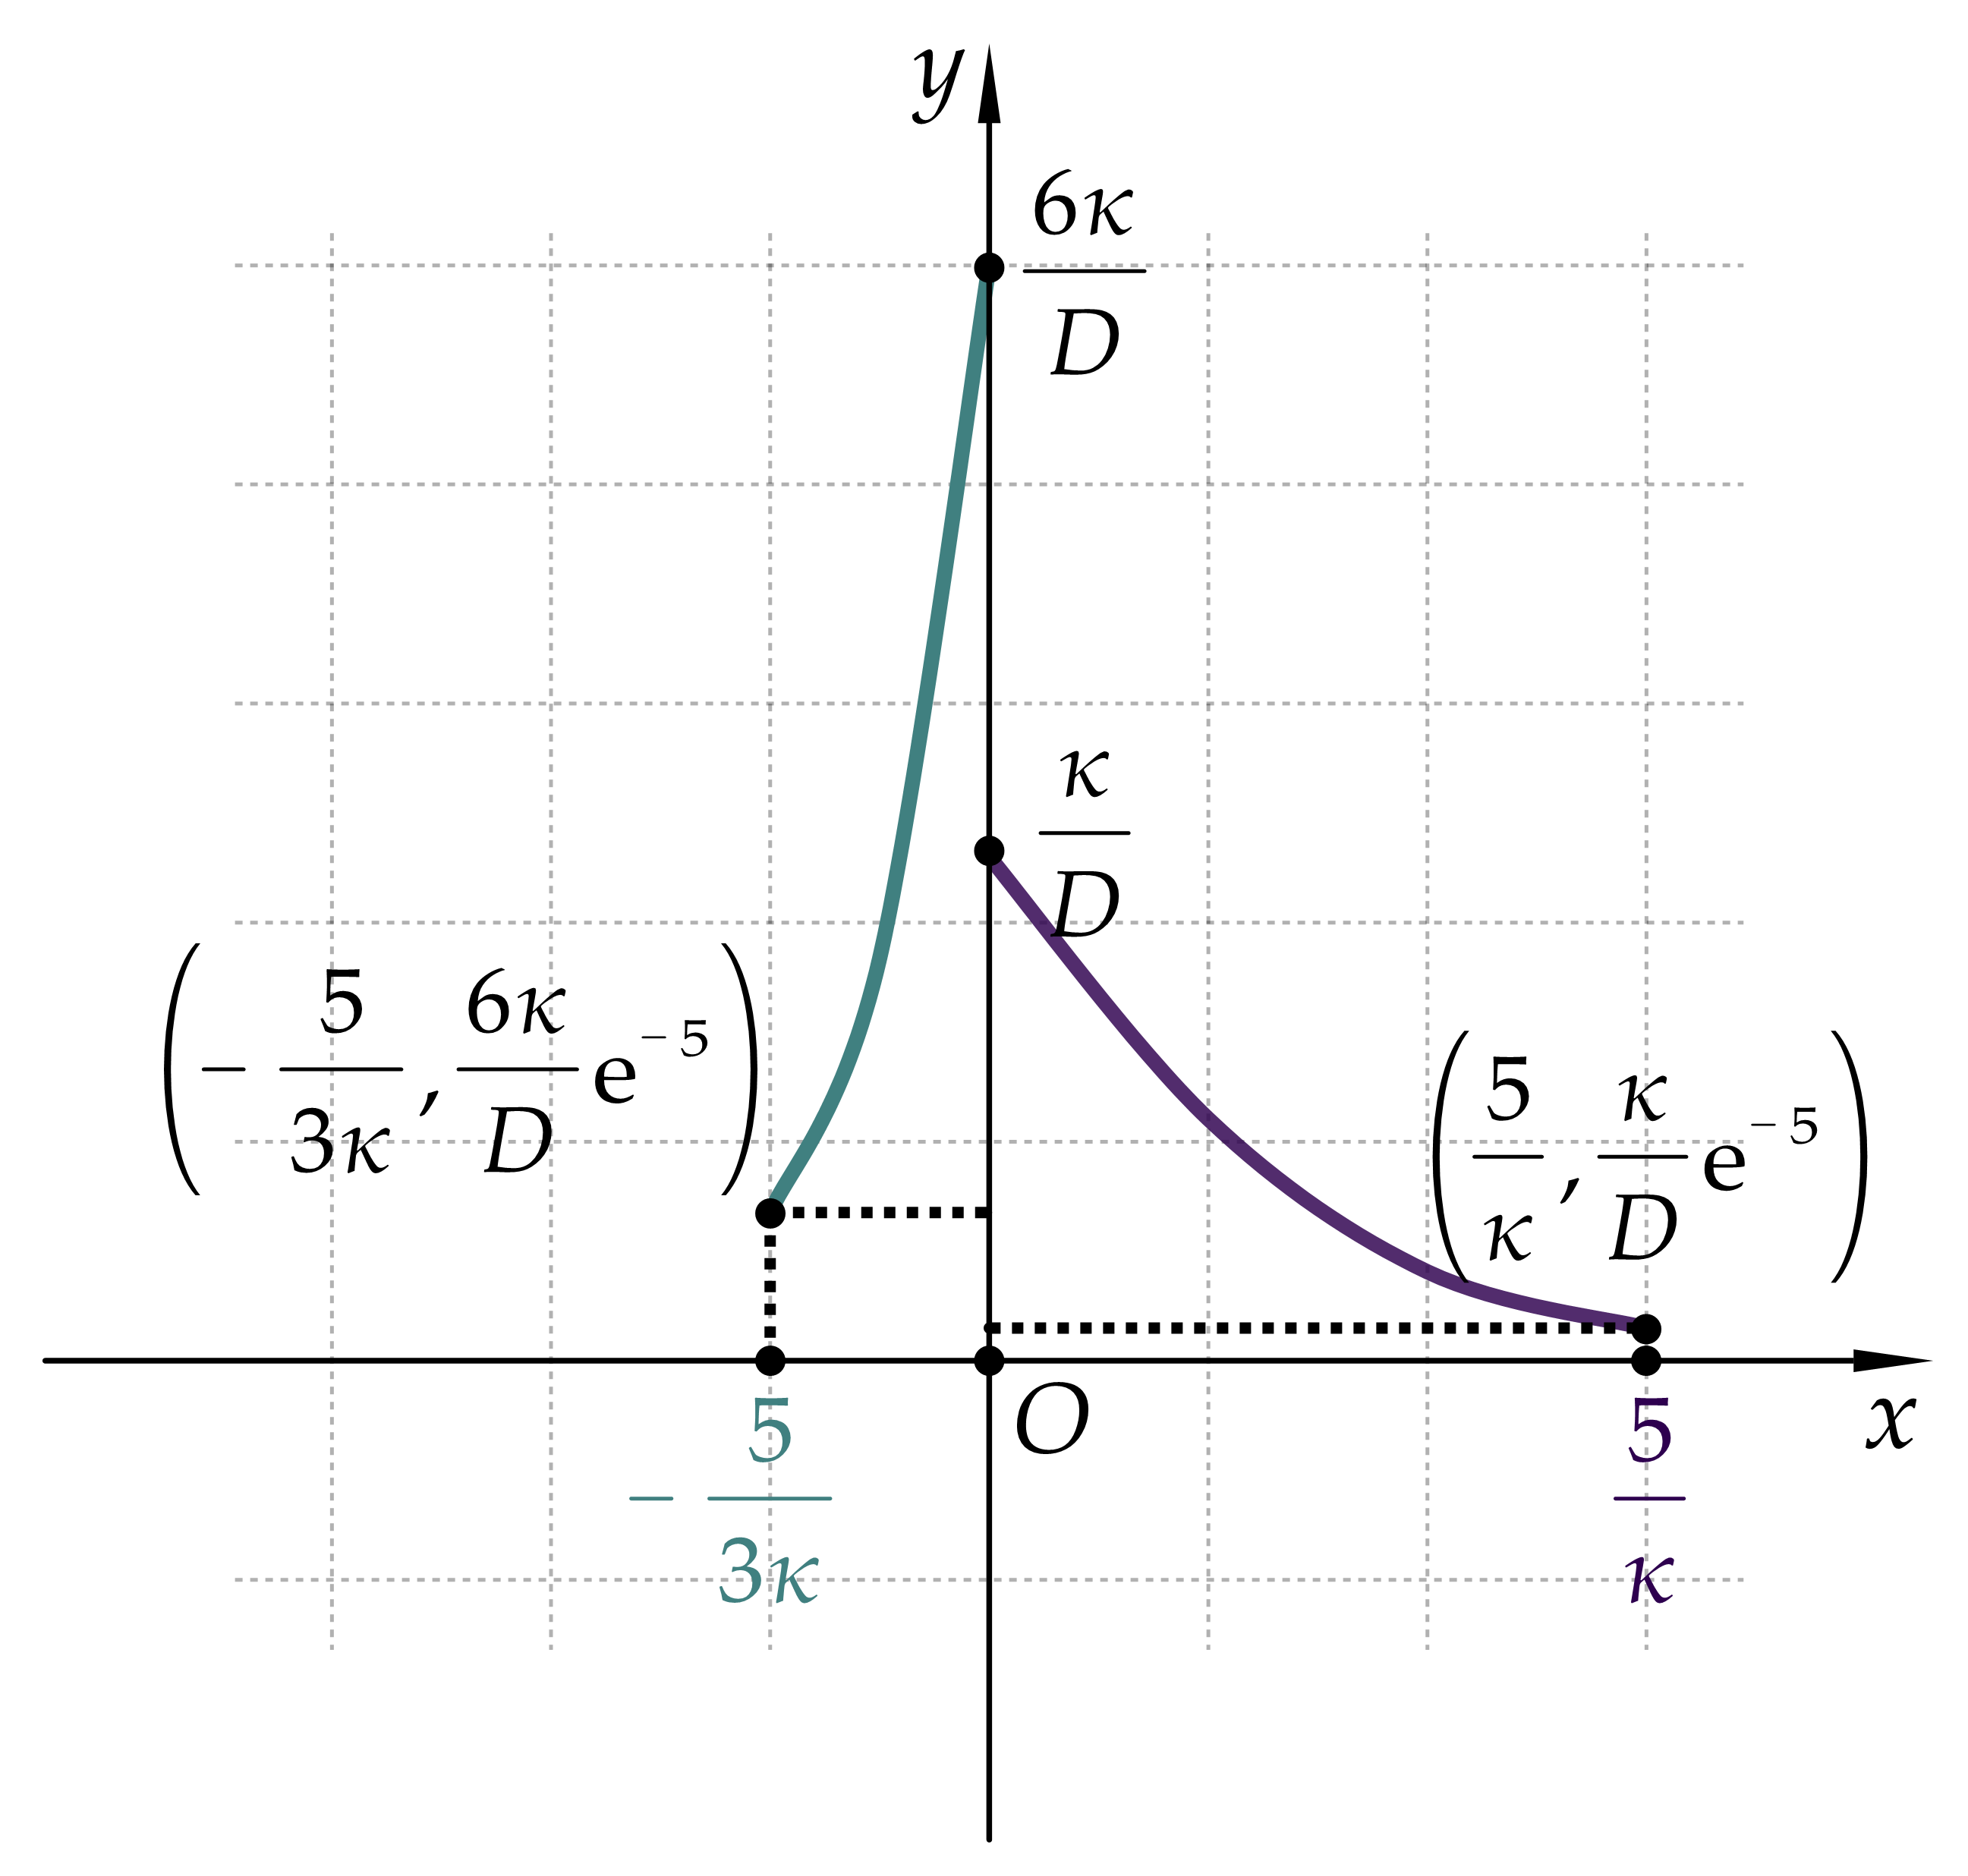
\includegraphics[scale=0.8]{figures/fig4.9-3.png}
            \end{figure}
        \end{enumerate}
    \end{solution}
\end{exercise}